\documentclass{article}

\usepackage[preprint]{neurips_2021}

\usepackage[utf8]{inputenc} % allow utf-8 input
\usepackage[T1]{fontenc}    % use 8-bit T1 fonts
\usepackage{hyperref}       % hyperlinks
\usepackage{url}            % simple URL typesetting
\usepackage{booktabs}       % professional-quality tables
\usepackage{amsfonts}       % blackboard math symbols
\usepackage{nicefrac}       % compact symbols for 1/2, etc.
\usepackage{microtype}      % microtypography
\usepackage{xcolor}         % colors
\usepackage{subfig,graphicx}
\usepackage[noabbrev,nameinlink, capitalise]{cleveref}
\usepackage[
backend=biber,
style=numeric,
]{biblatex}
\addbibresource{citations.bib}
\title{Analyzing ratings of Google Play Store applications}

\author{%
  Ivan Radonov \\
  \texttt{ivan.radonov@student.uni-tuebingen.de} \\
  }
\begin{document}

\maketitle

\begin{abstract}
  This study uses a dataset containing both free and paid apps from Google Play Store and looks at how users ratings differ between both categories. Further, the most popular paid app categories are explored and the relationship between application rating and the price, size, and last updated date is assessed.
\end{abstract}

\section{Introduction}

Google Play Store is the official app store for Android devices. Apps can be uploaded from certified users (developers) and can be downloaded from any user, provided that they meet the age restriction, their device fulfills all technical requirements, and they pay for it before use, in case the app is paid. App creators can decide whether their apps are free or paid. Any app can still have paid features inside it which are independent of its price.

A rating of an app provides a crowdsourced indicator of its quality \cite{mobileapprating}, hence it can be regarded as a key feature to optimize. To this end, android developers need to make some important decisions while developing an app regarding its other features, for example, whether the app should be paid and whether it should meet some size constraints. In this study, an app dataset from the Google Play Store was used to answer some of these questions and help Android developers make better decisions.

There exist similar studies, which focus on specific app categories, such as nutritional or finance apps \cite{nutritionalapps}, \cite{financialapps}. Other studies focus on sentiment analysis on the user reviews \cite{sentiment}. No studies were found which emphasize how the app price reflects user satisfaction.

\section{Methods}

\subsection{Origin and structure of app data}

The data was downloaded from Kaggle:
\begin{center}
    \url{https://www.kaggle.com/lava18/google-play-store-apps}
\end{center} It contains a snapshot of 13 characteristics from 10841 apps available in the Google Play Store as of August 2018. Notable features include:

- the app name, app category, rating, number of installations and reviews, type (paid or free), price in US dollars, size, and last updated date.

There are 34 app categories in total. The rating shows the average rating given by users of the app in the range from 1 (lowest) to 5 (highest). The app size is either given in KB or MB, or it varies with device.

\subsection{Data preprocessing}

Prior to conducting the analysis, the dataset was preprocessed. Missing values for some apps were imputed based on internet research. The columns containing the rating, number of reviews, number of installs, and the price were converted to numerical values. The app size was converted to the same unit (MB). To obtain the number of days since an app was last updated, the difference in days between the last updated date for the app and the last updated date for any app was calculated. Then, only apps updated in the last 1000 days were taken to remove outliers. In order to mitigate bias, apps with fewer than 20 reviews were removed from the analysis. Apps with missing ratings were also removed.

\subsection{Data analysis}

The dataset was split into free and paid apps. A two-sample Kolmogorov-Smirnov (KS) test was used to determine whether both samples are drawn from the same distributions. The KS test is a nonparametric test used for one-dimensional probability distributions \cite{kstest}. It can be either one-sample, where a sample is compared to a reference distribution, or two-sample, where two samples are compared. The test statistic is the maximum absolute difference of both cumulative distributions. The null hypothesis assumes both samples come from the same distribution. An implementation of the KS test is provided \verb+scipy+, a Python library for scientific computing \cite{scipy}.

All visualizations were done using Python's \verb+seaborn+ library, which is used to create statistical graphics \cite{seaborn}. Linear regression fits for different features were done using the built-in functionalities of the library.

The full data processing and analysis pipeline can be found in the \verb+RatingAnalysis.ipynb+ notebook.

\section{Results}

\subsection{Application price vs. rating}
\label{pricerating}
The rating distributions for both app types as well as the corresponding mean values are displayed in \cref{fig1}.

\begin{figure}[h]
    \centering
    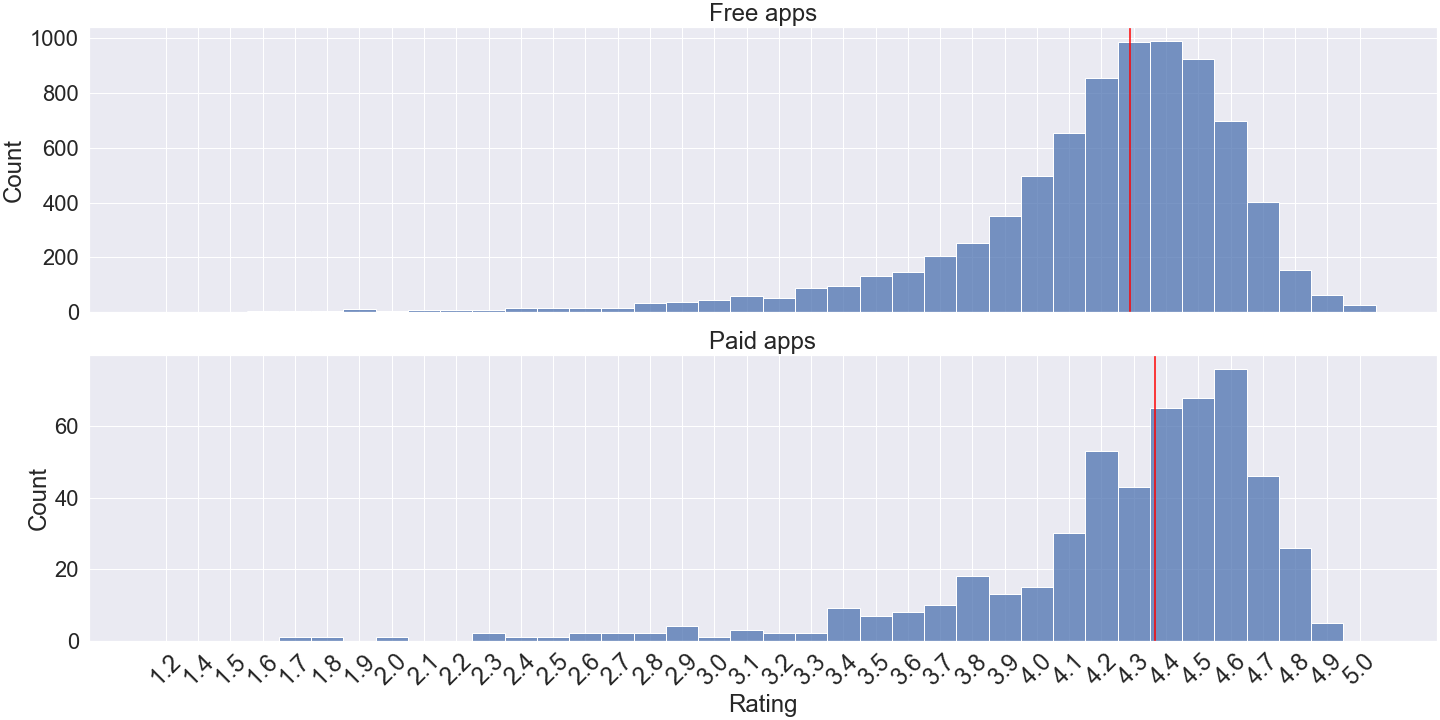
\includegraphics[scale=0.27]{figures/rating_distr.png}
    \caption{Rating distribution of free (top picture) and paid (bottom picture) apps, with corresponding rating means across apps given as vertical red lines. Apps with missing rating values or fewer than 20 reviews are not shown. The number of bins corresponds to the number of discrete rating values.}
    \label{fig1}
\end{figure}

As can be seen from this figure, the rating of the vast majority of the apps lies in the range from $3.5$ to $5$.

The Kolmogorov-Smirnov test returned a p-value of $1.22\times e^{-8}$ and a test statistic of $0.138$. The null hypothesis was thus rejected, and both samples were deemed different. This finding can be confirmed by \cref{fig1}, although both sample means are equal.

\subsection{Relationship between app rating and other features}

Further, the study aimed to find whether there exists a relationship between the rating of an app and some of its other features. To this end, the app size, price, and the last updated date were considered. \cref{fig2} visualizes the findings. Each subfigure shows a joint plot of rating and the other feature, with marginal plots on the top and left. 


\begin{figure}[h]\centering
\subfloat[App rating vs. price]{\label{a}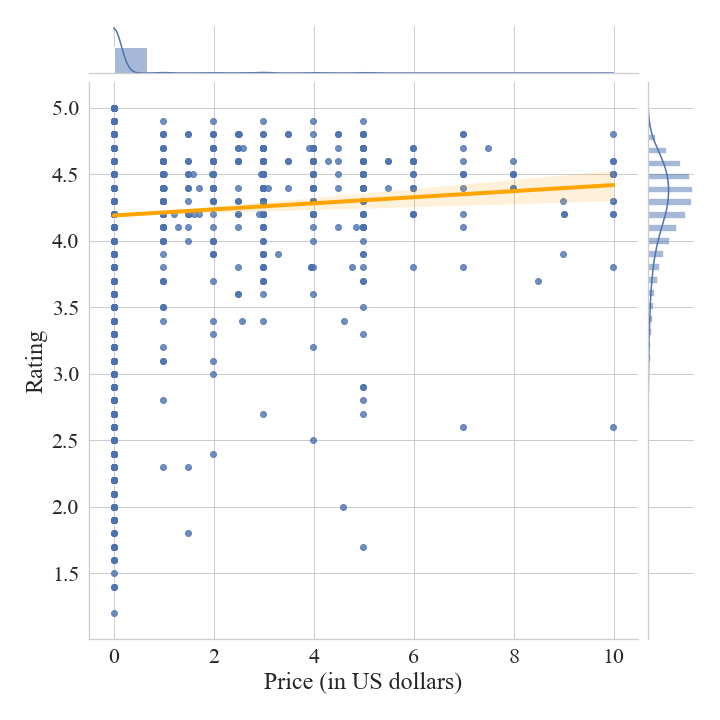
\includegraphics[width=.45\linewidth]{figures/price.png}}\hfill
\subfloat[App rating vs. size]{\label{b}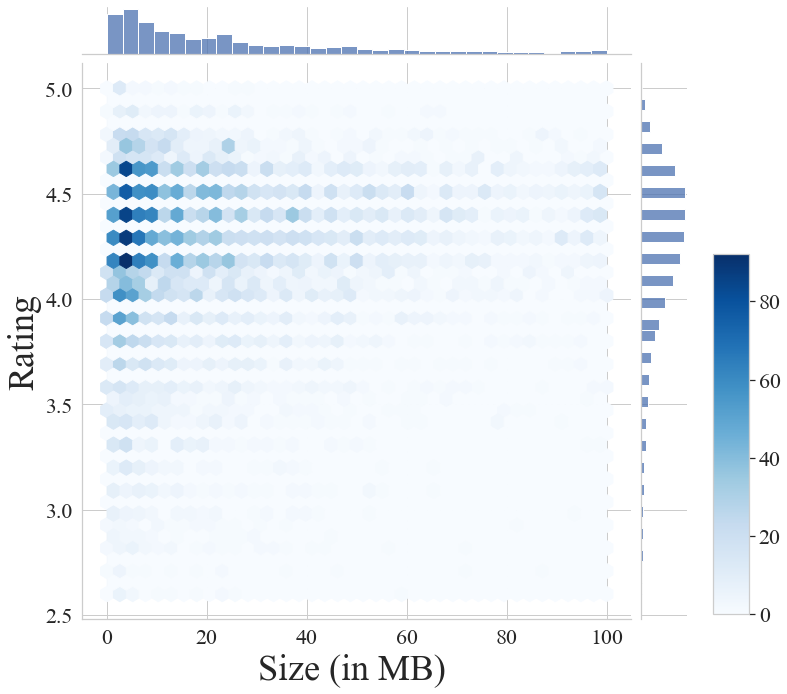
\includegraphics[width=.45\linewidth]{figures/size.png}}\par 
\subfloat[App rating vs. last updated time]{\label{c}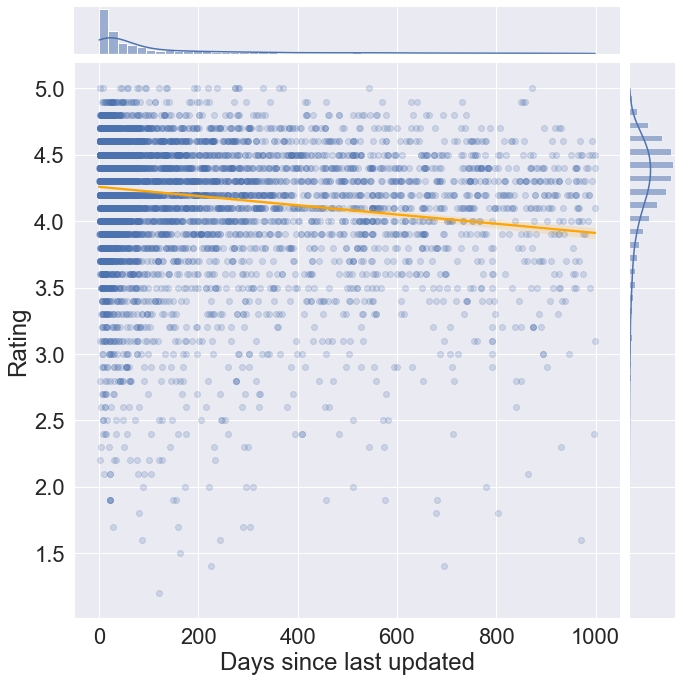
\includegraphics[width=.45\linewidth]{figures/updated.png}}
\caption{The relationship between app rating and three other features. In each figure, the top/left plots show the marginal distributions of that feature. Figure (a) compares the app rating to the last updated date. Figure (b) compares the rating to the app price, given in US dollars. Figure (c) shows a density plot of the rating and app size, given in MB. Darker values correspond to higher density. Orange lines in figures (a) and (b) show the best fitting line found by a standard linear regression model.}
\label{fig2}
\end{figure}

For all three said features, a standard linear regression model was used to determine a correlation. For the app price and last updated date, the best fitting line found by the model was plotted in \cref{fig2} as an orange line. For the app size, no strong relationship could be found, thus there was no relationship found. For this reason, only a density plot is shown. 


\section{Discussion}

The results from \cref{pricerating} imply that making an app paid can slightly improve its rating. Needless to say, this would decrease the user basis, so the price has to be chosen carefully.

The insights from \cref{fig2} can be summarized as follows: increasing an app's price has a beneficial influence on its rating. Apps that are updated more frequently receive substantially higher ratings. There was no substantial relationship found between the app size and its rating, although it can be seen that most apps are below 20 MB in size, which can serve as a guidance for the app scope.

Based on the result of this study, some suggestions can be given as to how to design Android applications: To achieve high ratings, an app should be frequently updated, of moderate size, and be paid, in case it provides some features missing in other similar apps.

Several limitations impeded achieving better results. First, since paid apps are affordable to fewer people, their ratings may be biased by the user profile. Further, both rating and number of installs are imperfect measures of app quality, since they don't tell e.g., how long the app was installed or if the ratings were honest, thus they are not perfect predictors of the app's profitability. Further studies may consider sentiment analysis on the user reviews, for which there are also available datasets.

\section{Conclusion}

In this report, app data from the Google Play Store was visualized and analyzed. It was found that paid applications receive slightly higher ratings. The relationships between an app's rating and its price, size, and last updated date were assessed and discussed. Key findings were that app rating increases with the price and update frequency. Several limitations of the data, applications and extensions of the analysis were pointed out.

\appendix
\printbibliography


\end{document}